\documentclass[11pt]{article}
\usepackage{amsmath}
\usepackage[utf8]{inputenc}
\usepackage{amsfonts,url,epsfig,breakurl}
%%% Document layout, margins
\usepackage{geometry}
\geometry{letterpaper, textwidth=6in, textheight=8.5in, marginparsep=1em}
%%% Section headings
\usepackage{sectsty}
\usepackage[normalem]{ulem}
\usepackage{booktabs}

%\setlength{\baselineskip}{40pt}

%\usepackage{hyperref}
\usepackage{todonotes}
\newcommand{\AG}[1]{\todo[inline,author=AG]{#1}}
\newcommand{\ag}[1]{\todo[size=\tiny]{ag: #1}{}}
\newcommand{\MV}[1]{\todo[inline,author=MV]{#1}}
\newcommand{\mv}[1]{\todo[size=\tiny]{mv: #1}{}}
\usepackage{verbatim}

\sectionfont{\sffamily\bfseries\upshape\large}
\subsectionfont{\sffamily\bfseries\upshape\normalsize}
\subsubsectionfont{\sffamily\mdseries\upshape\normalsize}
\makeatletter
\renewcommand\@seccntformat[1]{\csname the#1\endcsname.\quad}
\makeatother\renewcommand{\bibitem}{\vskip2pt\par\hangindent\parindent\hskip-\parindent}
\newcommand{\mme}{\mathbb{E}}

\makeatletter
\def\@maketitle{%
  \begin{center}%
  \let \footnote \thanks
    {\large \@title \par}%
    {\normalsize
      \begin{tabular}[t]{c}%
        \@author
      \end{tabular}\par}%
    {\small \@date}%
  \end{center}%
}
\makeatother


\title{\bf Quantifying Uncertainty in Prevalence Estimation Under Some Exponential Family Distribution \vspace{.1in}} 


%\author{Naa Odey Solomon, Gabriel A. Okyere, Elliot Owusu Addo  \vspace{.1in}}

\date{January, 2026}

\begin{document}\sloppy
	\maketitle

\begin{abstract}
	\noindent
Reliable estimation of disease prevalence is challenging when diagnostic tests yield continuous measurements and prevalence is low. Threshold-based approaches dichotomize outcomes, discarding information and ignoring classification uncertainty. We propose cutoff-free prevalence estimation using a two-component Gamma mixture model that directly models continuous diagnostic measurements. Maximum likelihood estimation via the EM algorithm is compared with Bayesian inference under objective priors, including a Uniform prior, Jeffreys’ prior and the maximum data information prior (MDIP). Simulation studies across varying sample sizes and component overlap show that EM estimation can be unstable in small samples, while Bayesian inference provides regularized and more stable uncertainty quantification. As sample size increases, the two approaches converge. The method offers a practical alternative to threshold-based prevalence estimation for rare-disease and limited-sample settings.
\end{abstract}





\section{Background}

Accurate estimation of disease prevalence is a central problem in epidemiology and public health, informing surveillance, resource allocation, and policy decisions. Prevalence is commonly estimated using diagnostic tests applied to population samples; however, uncertainty arising from diagnostic misclassification, sampling variability, and model assumptions can substantially distort inference, particularly when disease prevalence is low (Rogan \& Glaen, 1978; Joseph et al., 1995).
In applied practice, continuous diagnostic measurements are frequently dichotomized using fixed cut-off values to classify individuals as positive or negative. While this approach is operationally convenient and simple in estimating prevalence, it is well documented that dichotomization leads to loss of information, reduced statistical power, and biased estimation (Pepe, 2003; Altman \& Royston, 2006). These effects increase the overlap of diagnostic measurement distributions across latent subpopulations, especially when test sensitivity and specificity are imperfect or unknown.

Classical approaches to prevalence estimation typically rely on binary test outcomes and assume known or fixed diagnostic accuracy parameters. The Rogan-Gladen estimator and its extensions adjust observed prevalence using sensitivity and specificity estimates but ignore uncertainty in the quantities and may yield implausible estimates in small samples (Rogan \& Gladen, 1978; Reiczigel et al., 2010). These limitations have motivated the development of Bayesian methods that treat prevalence and diagnostic accuracy parameters as random variables, allowing uncertainty to be propagated coherently through the inferential process (Joseph et al., 1995; Johnson et al., 2018).


Recent Bayesian work has further emphasized the importance of avoiding dichotomization altogether by modeling continuous diagnostic measurements directly. Cutoff-free approaches preserve information and can improve inferential efficiency, particularly in low-prevalence settings (Bouman et al., 2020; Gelman \& Carpenter, 2020). Mixture models provide a natural framework for such analyses, representing observed measurements as arising from latent infected and uninfected subpopulations. Within this context, exponential family distributions are especially attractive due to their flexibility and interpretability for positive-valued biomedical data (McLachlan \& Peel, 2000).

Despite these advances, several important gaps remain. First, there is limited guidance on how prior choice affects uncertainty quantification in cutoff-free Bayesian prevalence estimation using continuous exponential family models. Objective priors are often recommended in the absence of strong prior information, yet their finite sample behavior in mixture-based prevalence estimation has not been systematically examined. Second, direct comparisons between Bayesian and frequentist inference in this setting remain sparse, particularly with respect to uncertainty stability and boundary behavior in small samples.

This paper addresses these gaps by proposing and evaluating a Bayesian cutoff-free framework for prevalence estimation based on Gamma mixture models. The Gamma distribution is well suited to modeling continuous diagnostic measurements that are strictly positive, such as antibody titers or biomarker concentrations (Pepe, 2003). We focus on uncertainty quantification under three objective prior specifications: uniform prior, Jeffreys prior, and the Maximum Data Information Prior (MDIP), and benchmark Bayesian inference against the classical Expectation-Maximum algorithm. The main contributions of this paper include setting up a Bayesian cutoff-free prevalence estimator using a two-component Gamma mixture model for continuous diagnostic data using the probabilistic programming language Stan (Carpenter et al., 2017; Stan Development Team, 2020) and evaluating Bayesian inference relative to classical estimation across a range of sample sizes. 

The remainder of the paper is organized as follows. Section 2 presents the model setting and inferential framework. Section 3 reports results from a simulation study. Section 4 discusses practical implications and limitations.



\section{Model Setting and Inferential Framework}
\subsection{Continuous Diagnostic Mixture Model}

Let $ Y_1, \cdots, Y_n $ denote continuous diagnostic measurements obtained from a sample of $n$ individuals. We assume that each observation arises from one of two latent subpopulations corresponding to the infected and uninfected individuals. Let $ \pi \in (0, 1) $ the prevalence be denoted as the probability that a randomly selected individuals belongs to the infected group. Conditional on latent infection status, the diagnostic measurement are modeled using gamma distributions. Specifically, we assume:

\begin{align*}
Y_i \mid Z_i = 1 \sim Gamma (\alpha_1, \beta_1), Y_i \mid Z_i = 0 \sim Gamma (\alpha_0, \beta_0) 
\end{align*}

Where $ Z_i \in {0,1}$ is a latent indicator of infection status, $\alpha_k$ and $ \beta_k$ denote the shape and scale parameters for group $k \in {0,1}.$

Marginally, the observed data follow a two-component Gamma mixture model with density

\begin{align*}
f(y_i \mid \theta) = \pi f_{1} (y_i \mid \alpha_1, \beta_1) + (1 - \pi) f_{0} (y_i \mid \alpha_0, \beta_0)
\end{align*}

where $\theta = (\pi, \alpha_1, \beta_1,\alpha_0, \beta_0).$ This formulation allows prevalence to be inferred directly from the distributional structure of the continuous diagnostic measurements, without imposing arbitrary cut-off points.

\subsection{Bayesian Inference and Prior Specification}

Inference is conducted within a Bayesian framework, treating all unknown parameters as random variables. The posterior distribution is proportional to the product of the likelihood and the prior distribution. 

\begin{align*}
	p(\theta \mid y) \propto p(y \mid \theta) \times p(\theta)
\end{align*}

\subsubsection*{\textbf{Likelihood}}

The likelihood can be expressed as the product of the marginal density,

\begin{align*}
	\ell (y_1 \mid \theta) = \prod_{i = 1}^{n}  \pi f_{1} (y_i \mid \alpha_1, \beta_1) + (1 - \pi) f_{0} (y_i \mid \alpha_0, \beta_0)
\end{align*}


\subsubsection*{\textbf{Prior}}

We considered three objective prior specifications, chosen to assess the sensitivity of the posterior inference to prior structure in the absence of strong external information.  First, Uniform prior $(0, 1)$ is assigned to prevalence ($\pi$) , as it is a natural starting point (Gelman \& Carpenter, 2020). Although simple and commonly used, it is known to be sensitive to parameterizing and truncation, making it useful benchmark for assessing prior induced variability. Second, Jeffrey's prior is employed due to its invariance under reparameterization and frequent use of objective Bayesian analysis. For the prevalence parameter $\pi$, the Jeffery's prior is derived from the Fisher information matrix, $P_j(\pi) \propto \sqrt{I(\pi)}, I(\pi)$ being the fisher information for $\pi$ (Jeffreys, 1961). To derive the Jeffreys prior for the prevalence parameter, consider the latent indicator formulation. Conditional on $\pi$, the latent variable $Z_1, \cdots, Z_n$ following an independent Bernoulli distribution. 

\[
Z_i \mid \pi \sim Bernoulli (\pi)
\]

The log-likelihood for $\pi$, condition on $Z = Z_1, \cdots, Z_n$ is 
\[
\ell (\pi) = \sum_{i = n}^{n}[Z_i log \pi +(1- Z_i) log(1 - \pi)].
\]

Proof: The first derivative is 
\[
\frac{\ell(\pi)}{\pi} = \sum_{i = 1}^{n} \left(  \frac{Z_i}{\pi} + \frac{1 - Z_i}{1 - \pi}
\right)
\]

Second derivative

\[
\frac{\ell(\pi)}{\pi^2} = \sum_{i = 1}^{n} \left(  \frac{Z_i}{\pi^2} + \frac{1 - Z_i}{(1 - \pi)^2}
\right)
\]

Taking expectation with respect to $Z_i \sim Bernoulli(\pi)$, the fisher information is


\[
I(\pi) = \mathbb{E} \left[\frac{\partial^2 \ell(\pi)}{\partial \pi ^2}\right] = n\left(\frac{1}{\pi} + \frac{1}{1 - \pi}\right) = \frac{n}{\pi (1 - \pi)}
\]

Thus, the Jeffrey's prior for the prevalence parameter is 

\begin{align}
	P_j (\pi) \propto \sqrt{\frac{1}{\pi (1- \pi)}}
\end{align}

This corresponds to the $Beta (0.5, 0.5)$ distribution.

We also considered the Maximum Data Information Prior, which is obtained by maximizing the expected Kullback-Leibler divergence between the posterior and the prior (Zellner, 1984; Singh \& Dey, 1994). 

\[
P_{MDIP} (\pi) \propto \exp \left[\mathbb{E}_{Z\mid\pi}[log p (Z \mid \pi)]\right]
\]


Hence, the MDIP for the prevalence parameter takes the form

\begin{align}
P_{MDIP}(\pi) \propto \exp \left[n[\pi log \pi + ( 1- \pi) log(1 - \pi)]\right]
\end{align}

\subsubsection*{\textbf{Posterior Computation}}

Posterior inference is performed using Hamiltonian Monte Carlo (HMC), which enables efficient exploration of the posterior distribution in moderately high-dimensional parameter spaces (Neal, 2011). Convergence is assessed using trace plots, effective sample sizes, and potential scale reduction factors.


\subsection{Classical Approach (EM Algorithm)}

For comparison, the prevalence parameter is also estimated via the expectation maximization algorithm under the same Gamma mixture specification. The EM framework treats the latent infection indicators as missing data and proceeds by iteratively maximizing the expected complete data log-likelihood (Dempster et al., 1977; McLachlan \& Peel, 2000). 
In the E-step, posterior membership probabilities are computed for each observation conditional on current parameter estimates. Specifically, the expected value of the latent indicator $Z_i$ is given by 

\[
\gamma_{i}^{t} = P(Z_i = 1 \mid y_i, \theta^{t} = \frac{\pi ^t f_1(y_i \mid \alpha_1, \beta_0)}{ \pi ^t f_1(y_1 \mid \alpha_1, \beta_1) + (1 - \pi)^t f_0 ( y_i \mid \alpha_0, \beta_0)} )
\]


In the M-step, parameter estimates are updated by maximizing the expected complete data log-likelihood. The prevalence estimate is updated as 

\[
\pi^{t+1} = \frac{1}{n} \sum_{i=1}^{n} \gamma_{i} ^{t}
\]

Iteration continues until convergence, assessed by changes in the observed data log-likelihood falling below a pre-specified tolerance. 

\section{Simulation Study \& Design}
A simulation study was conducted to evaluate the finite sample performance of the proposed Bayesian prevalence estimator and to assess the impact of prior specification on uncertainty quantification. Bayesian inference under different objective priors was compared with classical expectation-maximization under a common model specification. The primary focus was on bias, interval width, and inferential stability across varying sample sizes.

Data were generated from a two-component Gamma mixture model corresponding to infected and uninfected subpopulations. For each simulated dataset, observations were drawn independently from the marginal mixture density defined in Section 2. Parameter values were chosen to reflect partially overlapping diagnostic distributions, following the example in Bouman et al. (2020). Specifically, the infected subpopulation was modeled as $ \text{Gamma} (\alpha_1 = 4, \beta_1 = 1)$, while the uninfected subpopulation followed a  $\text{Gamma} (\alpha_0 = 1, \beta_1 = 1)$ distribution with prevalence $\pi = 0.08)$. Simulation experiments were conducted under sample sizes $n \in (50,500,1000)$. 


\subsection{Simulation Results}

In Figure 1, we present the sample performance for prevalence estimation under the EM algorithm and Bayesian inference using three prior specifications: uniform prior as the base prior, Jeffrey’s prior, and MDIP, an alternative prior to the uniform, across increasing sample sizes. The results show that Bayesian prevalence estimation techniques, specifically the Uniform prior, provide superior stability and uncertainty quantification in small samples relative to the EM algorithm, while maintaining the asymptotic agreement in large samples. Among the objective priors considered, the MDIP exhibits the most favorable bias-variance trade-off in low-sample settings. 

At the smallest sample size, n = 50, the EM algorithm shows a downward bias, with a mean estimate of 0.043 and a bias of -0.037. The corresponding interval includes the boundary at zero, indicating instability and poor precision in low-prevalence, small-sample settings. In contrast, Bayesian estimators demonstrate improved sample performance. Under the uniform prior, the posterior mean (0.075) is close to the true prevalence, with minimal bias; however, posterior uncertainty remains large, resulting in wide credible intervals. Jeffrey's prior produces a more traditional estimate (mean 0.048) with increased downward bias. The MDIP yields the most stable small-sample behavior, with a posterior mean of 0.067 and reduced bias (-0.013), reflecting stronger shrinkage toward the interior of the parameter space. 

\begin{figure}[htbp]
	\begin{small}
		\centerline{
			\begin{tabular}{lcccccccc}
				\toprule
				& \multicolumn{4}{c}{EM Algorithm} & \multicolumn{4}{c}{Uniform Prior} \\
				\cmidrule(lr){2-5} \cmidrule(lr){6-9}
				Sample Size & Mean & SD & Bias & 95\% Interval & Mean & SD & Bias & 95\% Interval \\
				\midrule
				50   & 0.043 & 0.050 & -0.037 & 0 -- 0.143     & 0.075 & 0.055 & -0.005 & 0 -- 0.181 \\
				500  & 0.069 & 0.019 & -0.010 & 0.033 -- 0.108 & 0.073 & 0.019 & -0.007 & 0.037 -- 0.111 \\
				1000 & 0.074 & 0.013 & -0.005 & 0.047 -- 0.101 & 0.075 & 0.014 & -0.005 & 0.048 -- 0.102 \\
				\midrule
				& \multicolumn{4}{c}{Jeffreys' Prior} & \multicolumn{4}{c}{MDIP} \\
				\cmidrule(lr){2-5} \cmidrule(lr){6-9}
				Sample Size & Mean & SD & Bias & 95\% Interval & Mean & SD & Bias & 95\% Interval \\
				\midrule
				50   & 0.048 & 0.049 & -0.032 & 0 -- 0.148     & 0.067 & 0.052 & -0.013 & 0 -- 0.167 \\
				500  & 0.070 & 0.019 & -0.010 & 0.034 -- 0.108 & 0.072 & 0.019 & -0.008 & 0.034 -- 0.108 \\
				1000 & 0.074 & 0.014 & -0.006 & 0.048 -- 0.103 & 0.075 & 0.013 & -0.005 & 0.049 -- 0.102 \\
				\bottomrule
			\end{tabular}
		}
	\end{small}
	\caption{\em Summary of inference from model with two-component Gamma mixture model, based on the information from Bouman et al. (2020): Reported are the posterior  mean, standard deviation (SD), bias, and 95\% credible interval across 1,000 replications for sample sizes $n = 50, 500,$ and $1000$. The true prevalence is $\pi = 0.08$.}
	\label{posterior1}
\end{figure}

As the sample size increases to n = 500, bias and variability decrease substantially across all methods. The posterior means under the Bayesian priors range from 0.070 to 0.073, with standard deviations that are nearly identical to those obtained using the EM algorithm. Interval estimates become narrower and are very centered around the true prevalence, indicating improved identifiability of the mixture components and reduced prior influence. 


At n = 1000, all estimators exhibit similar performance, with negligible bias and nearly identical uncertainty intervals. Differences across prior specifications and between Bayesian and frequentist approaches become minimal, confirming improved asymptotic properties under a correct model specification. It is also observed that Jeffreys' prior and the EM algorithm tend to have similar bias values as the sample size increases. Similarly, the Uniform prior and the MDIP tend to share similar characteristics as the sample size increases. Hence, the prevalence estimation of the uniform prior and EM algorithm would be studied. 

\subsubsection*{\textbf{Prior Sensitivity and Asymptotic Behavior}}

We evaluated the sensitivity of posterior inference for the prevalence parameter $\pi$ under three objective prior specifications: the Uniform prior, Jeffreys' prior, and the maximum data information prior(MDIP). Sensitivity was assessed across increasing sample sizes in order to examine both small-sample robustness and asymptotic behavior.
%
\begin{figure}[htbp]
	\centerline{ 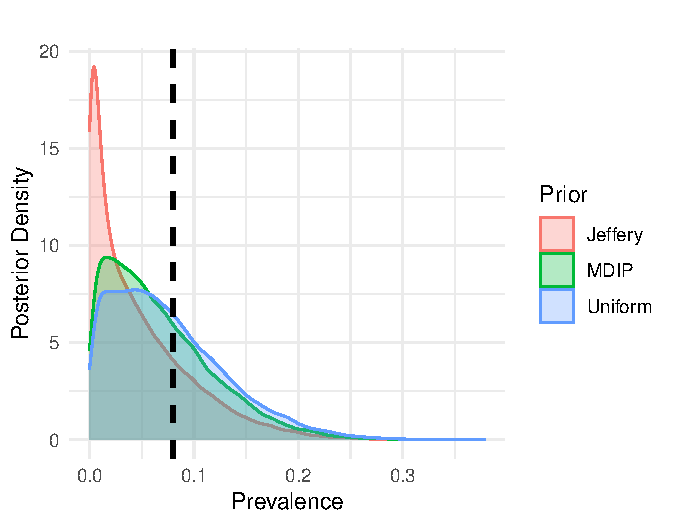
\includegraphics[width=.33\textwidth]{img/prior_sensitivity_50.pdf}
		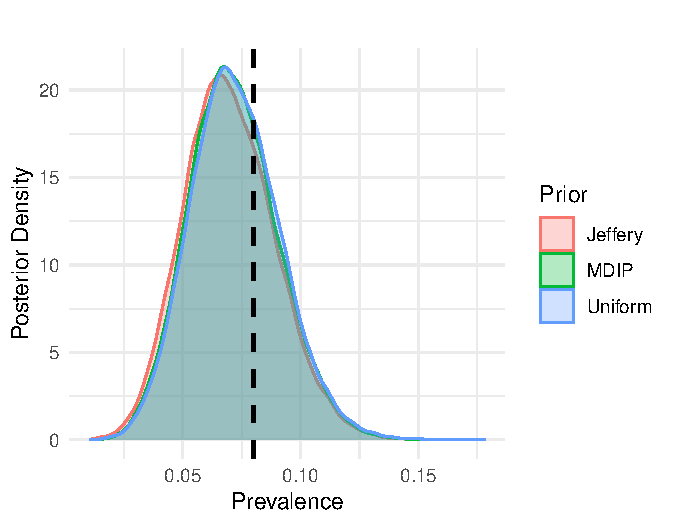
\includegraphics[width=.33\textwidth]{img/prior_sensitivity_500.pdf}
		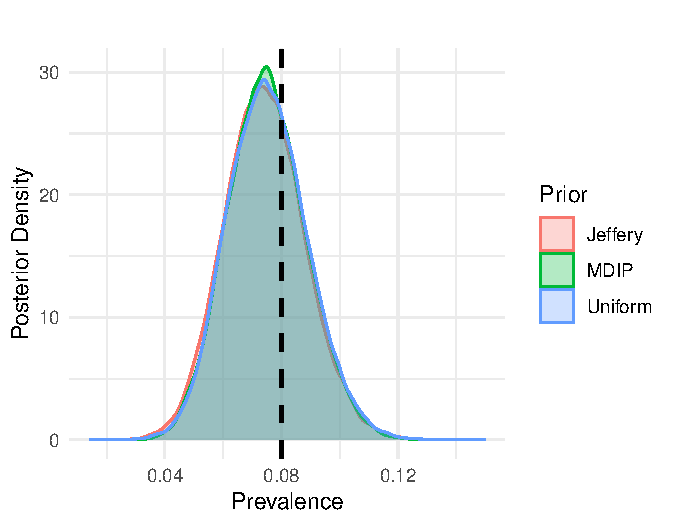
\includegraphics[width=.33\textwidth]{img/prior_sensitivity_1000.pdf}}
	\caption{\em Summary of inference from model with two-component Gamma mixture model, based on the example from Bouman et al. (2020): (a) posterior density of prevalence $\pi$, for $n = 50$; (b) posterior density of prevalence $\pi$, for $n = 500$; (c) posterior density of prevalence $\pi$, for $n = 1000$. Curves correspond to objective prior specifications (Uniform, Jeffreys, and MDIP). The model assumes fixed component distributions for infected and uninfected subpopulations and a common data-generating mechanism across replications.}
	\label{posterior2}
\end{figure}
%

In small sample $(n = 50)$, unassuming differences in posterior dispersion are observed across prior specifications. Although posterior means remain broadly aligned, the MDIP exhibits slightly greater concentration toward interior parameter values, consistent with its entropy-based construction, which discourages boundary mass. Jeffreys' prior, by contrast, allocates relatively more weight near the boundaries of the parameter space, potentially increasing dispersion when the data are weakly informative. Despite these differences in spread, posterior location remains stable across priors, suggesting that substantive conclusions regarding prevalence are not materially driven by prior choice.

As sample size increases $(n = 500)$ and $(n = 1000)$, posterior densities under all three priors become nearly indistinguishable. Differences in posterior means and credible intervals diminish rapidly, reflecting the decreasing influence of prior assumptions as information accumulates. This behavior is consistent with standard Bayesian asymptotic theory, under which the posterior distribution concentrates around the true parameter value and the likelihood progressively dominates inference under regularity conditions.


\subsubsection*{\textbf{Prevalence Performance Under Alternative Gamma Component Specification}}

Figure 3 reports the performance of prevalence estimation under alternative Gamma component parameter configurations, illustrating sensitivity to the degree of separation between infected and uninfected diagnostic distributions. Results are based on 10,000 simulated datasets with sample size (n = 5{,}000), ensuring that asymptotic behavior predominates over finite-sample variability.



\begin{figure}[htbp]
	\begin{small}
		\centerline{
			\begin{tabular}{lcccccc}
				\toprule
				& \multicolumn{3}{c}{EM Algorithm} & \multicolumn{3}{c}{Uniform Prior} \\
				\cmidrule(lr){2-4} \cmidrule(lr){5-7}
				Hyperparameters & Mean & SD & 95\% Interval & Mean & SD & 95\% Interval \\
				\midrule
				\multicolumn{7}{l}{\textbf{(a)} $\alpha_1=4$, $\beta_1=1$, $\alpha_0=1$, $\beta_0=1$} \\
				\midrule
				& 0.079 & 0.006 & 0.067 -- 0.092 & 0.080 & 0.006 & 0.068 -- 0.092 \\
				\midrule
				\multicolumn{7}{l}{\textbf{(b)} $\alpha_1=2$, $\beta_1=1$, $\alpha_0=10$, $\beta_0=1$} \\
				\midrule
				& 0.077 & 0.004 & 0.069 -- 0.086 & 0.078 & 0.004 & 0.069 -- 0.085 \\
				\bottomrule
			\end{tabular}
		}
	\end{small}
	\caption{\em Summary performance of prevalence estimators under alternative Gamma component specifications. Panel (a) corresponds to the configuration $(\alpha_1 = 4, \beta_1 = 1; \alpha_0 = 1, \beta_0 = 1)$, and Panel (b) corresponds to $(\alpha_1 = 2, \beta_1 = 1; \alpha_0 = 10, \beta_0 = 1)$. Reported quantities include the mean estimate, standard deviation (SD), and 95\% interval for the prevalence parameter $(\pi)$. Results are shown for the EM algorithm and Bayesian inference under the Uniform prior.}
	\label{posterior3}
\end{figure}

Under component parameter setting (a), corresponding to moderate overlap between components $(\alpha_1 = 4, \beta_1 = 1; \alpha_0 = 1, \beta_0 = 1)$, both the EM algorithm and Bayesian inference under the Uniform prior yield prevalence estimates that are effectively unbiased. The mean estimates (0.079 for EM and 0.080 for the Uniform prior) are close to the true prevalence, and the corresponding standard deviations and 95\% uncertainty intervals are nearly identical. This agreement reflects the large sample size and adequate component separation, under which both inferential paradigms are primarily likelihood-driven.

Under component parameter setting (b), which induces stronger separation between the latent subpopulations $(\alpha_1 = 2, \beta_1 = 1; \alpha_0 = 10, \beta_0 = 1)$, both methods again perform similarly. Standard deviations are reduced relative to setting (a), reflecting improved identifiability of the mixture components and greater information about the prevalence parameter. Bootstrap-based confidence intervals for the EM estimator closely align with Bayesian credible intervals, suggesting that asymptotic normality provides a satisfactory approximation in this regime.



%

\begin{figure}[htbp]
	\centerline{ 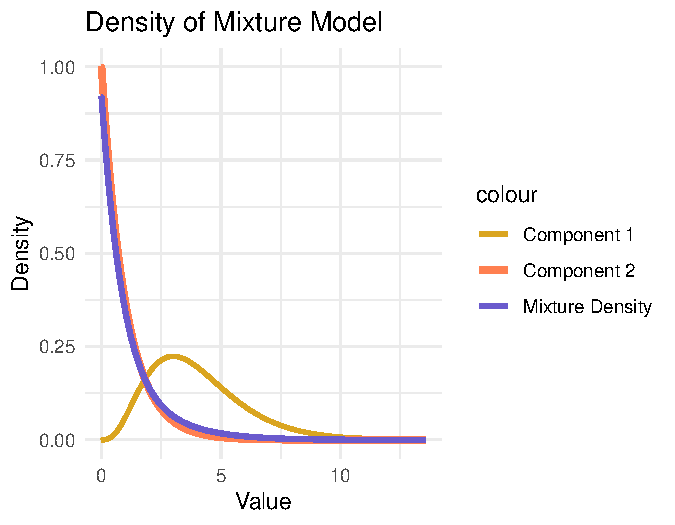
\includegraphics[width=.5\textwidth]{img/mixture_density.pdf}
		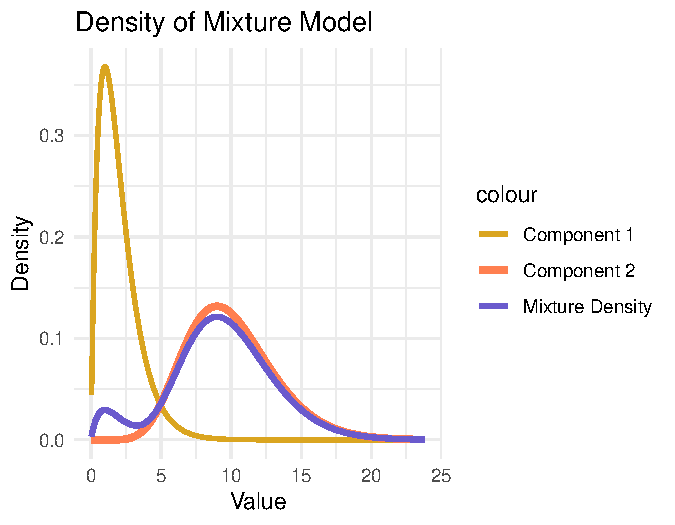
\includegraphics[width=.5\textwidth]{img/mixture_density_n.pdf}}
	\caption{\em Density of the two-component Gamma mixture model under alternative component parameter configurations: (a) component densities and resulting mixture density under moderate overlap between infected and uninfected subpopulations $(\alpha_1 = 4, \beta_1 = 1; \alpha_0 = 1, \beta_0 = 1)$; (b) component densities and resulting mixture density under increased separation between subpopulations $(\alpha_1 = 2, \beta_1 = 1; \alpha_0 = 10, \beta_0 = 1)$. In each panel, the individual component densities are displayed together with the implied marginal mixture density..}
	\label{posterior4}
\end{figure}
%
Taken together, these results indicate that when sample size is large and diagnostic distributions are sufficiently separated, differences between Bayesian and frequentist approaches become negligible. In such settings, uncertainty quantification is driven predominantly by the information content of the data rather than by prior specification or estimation strategy. These findings complement Table 1, where sample size varied, and reinforce that the principal advantages of the Bayesian cutoff-free framework emerge in low-prevalence or limited-sample contexts rather than in asymptotic regimes.


\section{Discussion}
This study investigated cutoff-free prevalence estimation using a two-component Gamma mixture model, comparing Bayesian inference under objective priors with classical maximum likelihood estimation via the EM algorithm. Modeling continuous diagnostic measurements directly avoids the information loss associated with dichotomization and yields stable inference across a range of sample sizes. In small samples and low-prevalence settings, Bayesian estimation, particularly under the MDIP and uniform priors, provides improved stability relative to EM while maintaining asymptotic agreement in larger samples.

The simulation results clarify the interaction between prevalence magnitude, component overlap, and sample size. When diagnostic distributions overlap substantially and sample size is limited, likelihood-based estimation becomes sensitive to boundary behavior and initialization. Bayesian regularization mitigates such degeneracy by constraining inference within the interior of the parameter space. As information accumulates, posterior distributions concentrate, and differences between inferential paradigms diminish, reflecting their shared likelihood foundation.

Prior sensitivity analysis indicates that conclusions regarding prevalence are not materially driven by objective prior choice. Although small-sample dispersion varies modestly across priors, posterior location remains stable, and prior influence decreases rapidly as sample size increases. These findings support the robustness of the cutoff-free Gamma mixture framework under reasonable non-informative prior specifications.

\subsection{Limitation of the statistical analysis}

Epidemiological prevalence estimation under mixture models entails latent structure and corresponding identification challenges. Several limitations of the present analysis therefore warrant consideration.

The simulation study assumes the correct model specification. In practice, diagnostic measurements may depart from the Gamma family, exhibiting heavier tails or multimodality. Such misspecification may bias prevalence estimates, particularly where identification depends on adequate separation between mixture components. In addition, certain simulation settings treat component parameters as fixed. In applied contexts, these quantities are typically unknown and must be estimated jointly, increasing model complexity and potentially aggravating identification difficulties.

Mixture models are inherently sensitive to overlap between latent subpopulations. When infected and uninfected distributions are weakly separated, prevalence is only weakly identified irrespective of the inferential paradigm. In such regimes, uncertainty is necessarily substantial and cannot be resolved by methodological choice alone. The analysis further assumes independence of observations and does not accommodate clustering, heterogeneous measurement error, or covariate structure; extensions to hierarchical or regression-based mixture formulations would be required for broader population applications.

Finally, although Hamiltonian Monte Carlo enables efficient posterior computation, mixture models may induce multimodal posterior surfaces. Careful convergence diagnostics and systematic sensitivity analyses remain essential in applied implementations.

\subsection{Practical implications }
Avoiding dichotomization of continuous diagnostic measurements preserves information and enhances inferential efficiency. Cutoff-based procedures discard distributional structure and may induce bias, particularly in low-prevalence settings. A mixture modeling framework incorporates classification uncertainty directly into prevalence estimation and provides a coherent alternative to threshold-based approaches.

Bayesian inference offers advantages in small samples and rare-disease contexts, where maximum likelihood estimation may exhibit instability or boundary solutions. Objective priors, including the Uniform prior and MDIP, supply regularization without imposing strong external assumptions and are therefore suitable when substantive prior knowledge is limited.

The results further emphasize the value of diagnostic separation. Greater assay discrimination reduces estimator variance and improves identifiability; in certain regimes, improvements in measurement precision may yield larger gains than increases in sample size alone.

In large samples with adequate component separation, differences between Bayesian and frequentist procedures become negligible. Under such conditions, the choice of inferential paradigm may reasonably be determined by computational considerations or reporting conventions rather than substantive performance differences.

The proposed framework contributes to reliable prevalence estimation in low-prevalence and limited-sample settings, where uncertainty quantification is particularly critical. Future work may extend this framework to hierarchical structures, covariate-dependent prevalence models, and broader classes of exponential family distributions.



\section*{References}

\noindent

\bibitem Bouman, J. A., Bonhoeffer, S., and Regoes, R. R. (2020).
Estimating seroprevalence with imperfect serological tests: a cutoff-free approach.
{\small \url{https://www.biorxiv.org/content/10.1101/2020.04.29.068999v2}}

\bibitem Carpenter, B., Gelman, A., Hoffman, M. D., Lee, D., Goodrich, B.,
Betancourt, M., Brubaker, M., Guo, J., Li, P., and Riddell, A. (2017).
Stan: A probabilistic programming language.
{\em Journal of Statistical Software} {\bf 76}(1), 1--32.
{\small \url{https://www.jstatsoft.org/article/view/v076i01}}

\bibitem Dempster, A. P., Laird, N. M., and Rubin, D. B. (1977).
Maximum likelihood from incomplete data via the EM algorithm.
{\em Journal of the Royal Statistical Society: Series B} {\bf 39}, 1--38.

\bibitem Gelman, A. (2006).
Prior distributions for variance parameters in hierarchical models.
{\em Bayesian Analysis} {\bf 1}, 515--533.

\bibitem Gelman, A., Chew, G., and Shnaidman, M. (2004).
Bayesian analysis of serial dilution assays.
{\em Biometrics} {\bf 60}, 407--417.

\bibitem Gustafson, P. (2003).
{\em Measurement Error and Misclassification in Statistics and Epidemiology:
	Impacts and Bayesian Adjustments}. Boca Raton: CRC Press.

\bibitem McLachlan, G., and Peel, D. (2000).
{\em Finite Mixture Models}. New York: Wiley.

\bibitem Robert, C. P. (2007).
{\em The Bayesian Choice: From Decision-Theoretic Foundations to Computational Implementation}. 2nd ed. New York: Springer.

\bibitem Kass, R. E., and Wasserman, L. (1996).
The selection of prior distributions by formal rules.
{\em Journal of the American Statistical Association} {\bf 91}, 1343--1370.

\bibitem Jeffreys, H. (1946).
An invariant form for the prior probability in estimation problems.
{\em Proceedings of the Royal Society of London Series A} {\bf 186}, 453--461.

\bibitem Bernardo, J. M. (1979).
Reference posterior distributions for Bayesian inference.
{\em Journal of the Royal Statistical Society: Series B} {\bf 41}, 113--147.

\bibitem Carpenter, B., Gelman, A., Hoffman, M. D., Lee, D., Goodrich, B.,
Betancourt, M., Brubaker, M., Guo, J., Li, P., and Riddell, A. (2017).
Stan: A probabilistic programming language.
{\em Journal of Statistical Software} {\bf 76}(1), 1--32.

\bibitem Stan Development Team (2023).
{\em Stan User's Guide}.
{\small \url{https://mc-stan.org}}

\bibitem Liu, Y., Gelman, A., and Zheng, T. (2015).
Simulation-efficient shortest probability intervals.
{\em Statistics and Computing} {\bf 25}, 809--819.

\bibitem Greenland, S. (2009).
Bayesian perspectives for epidemiologic research: Bias analysis via missing-data methods.
{\em International Journal of Epidemiology} {\bf 38}, 1662--1673.

\bibitem Gigerenzer, G., Gaissmaier, W., Kurz-Milcke, E., Schwartz, L. M.,
and Woloshin, S. (2007).
Helping doctors and patients make sense of health statistics.
{\em Psychological Science in the Public Interest} {\bf 8}, 53--96.


\pagebreak
\appendix

\section{Stan programs}

\subsection{Model with Uniform Prior}

\vspace{-\baselineskip}
\begin{small}
	\begin{quotation}\noindent
		\verbatiminput{Stan-Code/Uniform.stan}
	\end{quotation}
\end{small}


\subsection{Model with Jeffrey's Prior}

\vspace{-\baselineskip}
\begin{small}
	\begin{quotation}\noindent
		\verbatiminput{Stan-Code/Jeff.stan}
	\end{quotation}
\end{small}

\subsection{Model with Maximum Data Information Prior}

\vspace{-\baselineskip}
\begin{small}
	\begin{quotation}\noindent
		\verbatiminput{Stan-Code/MDIP.stan}
	\end{quotation}
\end{small}



\end{document}


